\documentclass[journal,twoside,web]{ieeecolor}
\usepackage{generic}
\usepackage{cite}
\usepackage{amsmath,amssymb,amsfonts}
\usepackage{algorithmic}
\usepackage{graphicx}
\usepackage{algorithm,algorithmic}
\usepackage{hyperref}
\hypersetup{hidelinks=true}
\usepackage{textcomp}
\usepackage{orcidlink}
\def\BibTeX{{\rm B\kern-.05em{\sc i\kern-.025em b}\kern-.08em
    T\kern-.1667em\lower.7ex\hbox{E}\kern-.125emX}}
\markboth{\hskip25pc IEEE TRANSACTIONS ON MEDICAL IMAGING}
{Sheth \MakeLowercase{\textit{et al.}}: A DVT-Inspired 3D Transformer Bottleneck}

\begin{document}

\title{A DVT-Inspired 3D Transformer Bottleneck for Zero-Shot Self-Supervised Denoising of Two-Photon Calcium Imaging Video}

\author{Aagam Sheth \orcidlink{0009-0000-5499-0394}, and Jayendra Bhalodiya \orcidlink{0000-0001-6540-6835}
\thanks{This paragraph of the first footnote will contain the date on 
which you submitted your paper for review. It will also contain support 
information, including sponsor and financial support acknowledgment. For 
example, ``This work was supported in part by the U.S. Department of 
Commerce under Grant 123456.'' }
\thanks{Aagam Sheth and Jayendra Bhalodiya are with the School of Engineering and Applied Science, Ahmedabad University, Ahmedabad, Gujarat 380015, India (e-mail: aagam.s6@ahduni.edu.in; jayendra.bhalodiya@ahduni.edu.in).}
\thanks{The source code will be released at https://github.com/Aagam41/DL\_2026\_FMIDenoising.}
\thanks{Digital Object Identifier XX.XXXX/XXXX.2026.XXXXXXX}}

\maketitle

\begin{abstract}
Lorem ipsum dolor sit amet consectetur adipiscing elit quisque faucibus ex sapien vitae pellentesque sem placerat in id cursus mi pretium tellus duis convallis tempus leo eu aenean sed diam urna tempor pulvinar vivamus fringilla lacus nec metus bibendum egestas iaculis massa nisl malesuada lacinia integer nunc posuere ut hendrerit semper vel class aptent taciti sociosqu ad litora torquent per conubia nostra inceptos himenaeos orci varius natoque penatibus et magnis dis parturient montes nascetur ridiculus mus donec rhoncus eros lobortis nulla molestie mattis scelerisque maximus eget fermentum odio phasellus non purus est efficitur laoreet mauris pharetra vestibulum fusce dictum risus blandit quis suspendisse aliquet nisi sodales consequat magna ante condimentum neque at luctus nibh finibus facilisis dapibus etiam interdum tortor ligula congue sollicitudin erat viverra ac tincidunt nam porta elementum a enim euismod quam justo lectus commodo augue arcu dignissim velit aliquam imperdiet mollis nullam volutpat porttitor ullamcorper rutrum gravida.
\end{abstract}

\begin{IEEEkeywords}
Blind-spot networks, Noise2Void, self-supervised learning, calcium imaging, transformer bottleneck, denoising.
\end{IEEEkeywords}

\section{Introduction}
\label{sec:introduction}
Lorem ipsum dolor sit amet consectetur adipiscing elit. Quisque faucibus ex sapien vitae pellentesque sem placerat. In id cursus mi pretium tellus duis convallis. Tempus leo eu aenean sed diam urna tempor. Pulvinar vivamus fringilla lacus nec metus bibendum egestas. Iaculis massa nisl malesuada lacinia integer nunc posuere. Ut hendrerit semper vel class aptent taciti sociosqu. Ad litora torquent per conubia nostra inceptos himenaeos.

Lorem ipsum dolor sit amet consectetur adipiscing elit. Quisque faucibus ex sapien vitae pellentesque sem placerat. In id cursus mi pretium tellus duis convallis. Tempus leo eu aenean sed diam urna tempor. Pulvinar vivamus fringilla lacus nec metus bibendum egestas. Iaculis massa nisl malesuada lacinia integer nunc posuere. Ut hendrerit semper vel class aptent taciti sociosqu. Ad litora torquent per conubia nostra inceptos himenaeos.

Lorem ipsum dolor sit amet consectetur adipiscing elit. Quisque faucibus ex sapien vitae pellentesque sem placerat. In id cursus mi pretium tellus duis convallis. Tempus leo eu aenean sed diam urna tempor. Pulvinar vivamus fringilla lacus nec metus bibendum egestas. Iaculis massa nisl malesuada lacinia integer nunc posuere. Ut hendrerit semper vel class aptent taciti sociosqu. Ad litora torquent per conubia nostra inceptos himenaeos.

Lorem ipsum dolor sit amet consectetur adipiscing elit. Quisque faucibus ex sapien vitae pellentesque sem placerat. In id cursus mi pretium tellus duis convallis. Tempus leo eu aenean sed diam urna tempor. Pulvinar vivamus fringilla lacus nec metus bibendum egestas. Iaculis massa nisl malesuada lacinia integer nunc posuere. Ut hendrerit semper vel class aptent taciti sociosqu. Ad litora torquent per conubia nostra inceptos himenaeos.


\section{Related Work}
\subsection{Self-Supervised Denoising and Blind-Spot Networks}


\section{Method}
\label{sec:guidelines}

\subsection{Types of Graphics}
The following list outlines the different types of graphics published in 
IEEE journals. They are categorized based on their construction, and use of 
color/shades of gray:

\subsubsection{Color/Grayscale figures}
{Figures that are meant to appear in color, or shades of black/gray. Such 
figures may include photographs, illustrations, multicolor graphs, and 
flowcharts.}

\subsubsection{Line Art figures}
{Figures that are composed of only black lines and shapes. These figures 
should have no shades or half-tones of gray, only black and white.}

\subsubsection{Author photos}
{Head and shoulders shots of authors that appear at the end of our papers. }

\subsubsection{Tables}
{Data charts which are typically black and white, but sometimes include 
color.}

\begin{table}
\caption{Units for Magnetic Properties}
\label{table}
\setlength{\tabcolsep}{3pt}
\begin{tabular}{|p{25pt}|p{75pt}|p{115pt}|}
\hline
Symbol& 
Quantity& 
Conversion from Gaussian and \par CGS EMU to SI $^{\mathrm{a}}$ \\
\hline
$\Phi $& 
magnetic flux& 
1 Mx $\to  10^{-8}$ Wb $= 10^{-8}$ V$\cdot $s \\
$B$& 
magnetic flux density, \par magnetic induction& 
1 G $\to  10^{-4}$ T $= 10^{-4}$ Wb/m$^{2}$ \\
$H$& 
magnetic field strength& 
1 Oe $\to  10^{3}/(4\pi )$ A/m \\
$m$& 
magnetic moment& 
1 erg/G $=$ 1 emu \par $\to 10^{-3}$ A$\cdot $m$^{2} = 10^{-3}$ J/T \\
$M$& 
magnetization& 
1 erg/(G$\cdot $cm$^{3}) =$ 1 emu/cm$^{3}$ \par $\to 10^{3}$ A/m \\
4$\pi M$& 
magnetization& 
1 G $\to  10^{3}/(4\pi )$ A/m \\
$\sigma $& 
specific magnetization& 
1 erg/(G$\cdot $g) $=$ 1 emu/g $\to $ 1 A$\cdot $m$^{2}$/kg \\
$j$& 
magnetic dipole \par moment& 
1 erg/G $=$ 1 emu \par $\to 4\pi \times  10^{-10}$ Wb$\cdot $m \\
$J$& 
magnetic polarization& 
1 erg/(G$\cdot $cm$^{3}) =$ 1 emu/cm$^{3}$ \par $\to 4\pi \times  10^{-4}$ T \\
$\chi , \kappa $& 
susceptibility& 
1 $\to  4\pi $ \\
$\chi_{\rho }$& 
mass susceptibility& 
1 cm$^{3}$/g $\to  4\pi \times  10^{-3}$ m$^{3}$/kg \\
$\mu $& 
permeability& 
1 $\to  4\pi \times  10^{-7}$ H/m \par $= 4\pi \times  10^{-7}$ Wb/(A$\cdot $m) \\
$\mu_{r}$& 
relative permeability& 
$\mu \to \mu_{r}$ \\
$w, W$& 
energy density& 
1 erg/cm$^{3} \to  10^{-1}$ J/m$^{3}$ \\
$N, D$& 
demagnetizing factor& 
1 $\to  1/(4\pi )$ \\
\hline
\multicolumn{3}{p{251pt}}{Vertical lines are optional in tables. Statements that serve as captions for 
the entire table do not need footnote letters. }\\
\multicolumn{3}{p{251pt}}{$^{\mathrm{a}}$Gaussian units are the same as cg emu for magnetostatics; Mx 
$=$ maxwell, G $=$ gauss, Oe $=$ oersted; Wb $=$ weber, V $=$ volt, s $=$ 
second, T $=$ tesla, m $=$ meter, A $=$ ampere, J $=$ joule, kg $=$ 
kilogram, H $=$ henry.}
\end{tabular}
\label{tab1}
\end{table}

\subsection{Multipart figures}
Figures compiled of more than one sub-figure presented side-by-side, or 
stacked. If a multipart figure is made up of multiple figure
types (one part is lineart, and another is grayscale or color) the figure 
should meet the stricter guidelines.

\subsection{File Formats For Graphics}\label{formats}
Format and save your graphics using a suitable graphics processing program 
that will allow you to create the images as PostScript (PS), Encapsulated 
PostScript (.EPS), Tagged Image File Format (.TIFF), Portable Document 
Format (.PDF), Portable Network Graphics (.PNG), or Metapost (.MPS), sizes them, and adjusts 
the resolution settings. When 
submitting your final paper, your graphics should all be submitted 
individually in one of these formats along with the manuscript.

\subsection{Sizing of Graphics}
Most charts, graphs, and tables are one column wide (3.5 inches/88 
millimeters/21 picas) or page wide (7.16 inches/181 millimeters/43 
picas). The maximum depth a graphic can be is 8.5 inches (216 millimeters/54
picas). When choosing the depth of a graphic, please allow space for a 
caption. Figures can be sized between column and page widths if the author 
chooses, however it is recommended that figures are not sized less than 
column width unless when necessary. 

There is currently one publication with column measurements that do not 
coincide with those listed above. Proceedings of the IEEE has a column 
measurement of 3.25 inches (82.5 millimeters/19.5 picas). 

The final printed size of author photographs is exactly
1 inch wide by 1.25 inches tall (25.4 millimeters$\,\times\,$31.75 millimeters/6 
picas$\,\times\,$7.5 picas). Author photos printed in editorials measure 1.59 inches 
wide by 2 inches tall (40 millimeters$\,\times\,$50 millimeters/9.5 picas$\,\times\,$12 
picas).

\subsection{Resolution }
The proper resolution of your figures will depend on the type of figure it 
is as defined in the ``Types of Figures'' section. Author photographs, 
color, and grayscale figures should be at least 300dpi. Line art, including 
tables should be a minimum of 600dpi.

\subsection{Vector Art}
In order to preserve the figures' integrity across multiple computer 
platforms, we accept files in the following formats: .EPS/.PDF/.PS. All 
fonts must be embedded or text converted to outlines in order to achieve the 
best-quality results.

\subsection{Color Space}
The term color space refers to the entire sum of colors that can be 
represented within the said medium. For our purposes, the three main color 
spaces are Grayscale, RGB (red/green/blue) and CMYK 
(cyan/magenta/yellow/black). RGB is generally used with on-screen graphics, 
whereas CMYK is used for printing purposes.

All color figures should be generated in RGB or CMYK color space. Grayscale 
images should be submitted in Grayscale color space. Line art may be 
provided in grayscale OR bitmap colorspace. Note that ``bitmap colorspace'' 
and ``bitmap file format'' are not the same thing. When bitmap color space 
is selected, .TIF/.TIFF/.PNG are the recommended file formats.

\subsection{Accepted Fonts Within Figures}
When preparing your graphics IEEE suggests that you use of one of the 
following Open Type fonts: Times New Roman, Helvetica, Arial, Cambria, and 
Symbol. If you are supplying EPS, PS, or PDF files all fonts must be 
embedded. Some fonts may only be native to your operating system; without 
the fonts embedded, parts of the graphic may be distorted or missing.

A safe option when finalizing your figures is to strip out the fonts before 
you save the files, creating ``outline'' type. This converts fonts to 
artwork what will appear uniformly on any screen.

\subsection{Using Labels Within Figures}

\subsubsection{Figure Axis labels }
Figure axis labels are often a source of confusion. Use words rather than 
symbols. As an example, write the quantity ``Magnetization,'' or 
``Magnetization M,'' not just ``M.'' Put units in parentheses. Do not label 
axes only with units. As in Fig. 1, for example, write ``Magnetization 
(A/m)'' or ``Magnetization (A$\cdot$m$^{-1}$),'' not just ``A/m.'' Do not label axes with a ratio of quantities and 
units. For example, write ``Temperature (K),'' not ``Temperature/K.'' 

Multipliers can be especially confusing. Write ``Magnetization (kA/m)'' or 
``Magnetization (10$^{3}$ A/m).'' Do not write ``Magnetization 
(A/m)$\,\times\,$1000'' because the reader would not know whether the top 
axis label in Fig. 1 meant 16000 A/m or 0.016 A/m. Figure labels should be 
legible, approximately 8 to 10 point type.

\subsubsection{Subfigure Labels in Multipart Figures and Tables}
Multipart figures should be combined and labeled before final submission. 
Labels should appear centered below each subfigure in 8 point Times New 
Roman font in the format of (a) (b) (c). 

\subsection{File Naming}
Figures (line artwork or photographs) should be named starting with the 
first 5 letters of the author's last name. The next characters in the 
filename should be the number that represents the sequential 
location of this image in your article. For example, in author 
``Anderson's'' paper, the first three figures would be named ander1.tif, 
ander2.tif, and ander3.ps.

Tables should contain only the body of the table (not the caption) and 
should be named similarly to figures, except that `.t' is inserted 
in-between the author's name and the table number. For example, author 
Anderson's first three tables would be named ander.t1.tif, ander.t2.ps, 
ander.t3.eps.

Author photographs should be named using the first five characters of the 
pictured author's last name. For example, four author photographs for a 
paper may be named: oppen.ps, moshc.tif, chen.eps, and duran.pdf.

If two authors or more have the same last name, their first initial(s) can 
be substituted for the fifth, fourth, third$\ldots$ letters of their surname 
until the degree where there is differentiation. For example, two authors 
Michael and Monica Oppenheimer's photos would be named oppmi.tif, and 
oppmo.eps.

\subsection{Referencing a Figure or Table Within Your Paper}
When referencing your figures and tables within your paper, use the 
abbreviation ``Fig.'' even at the beginning of a sentence. Do not abbreviate 
``Table.'' Tables should be numbered with Roman Numerals.

\subsection{Submitting Your Graphics}
Because IEEE will do the final formatting of your paper,
you do not need to position figures and tables at the top and bottom of each 
column. In fact, all figures, figure captions, and tables can be placed at 
the end of your paper. In addition to, or even in lieu of submitting figures 
within your final manuscript, figures should be submitted individually, 
separate from the manuscript in one of the file formats listed above in 
Section \ref{formats}. Place figure captions below the figures; place table titles 
above the tables. Please do not include captions as part of the figures, or 
put them in ``text boxes'' linked to the figures. Also, do not place borders 
around the outside of your figures.

\subsection{Color Processing/Printing in IEEE Journals}
All IEEE Transactions, Journals, and Letters allow an author to publish color figures on IEEE Xplore at no charge, and automatically convert them to grayscale for print versions. In most journals, figures and tables may alternatively be printed in color if an author chooses to do so. Please note that this service comes at an extra expense to the author. If you intend to have print color graphics, you will have the opportunity to indicate this in the Author Gateway and will be contacted by PubOps to confirm the charges. Online-only journals will have their figures appear in color, free of charge 

\section{Conclusion}
A conclusion section is not required. Although a conclusion may review the 
main points of the paper, do not replicate the abstract as the conclusion. A 
conclusion might elaborate on the importance of the work or suggest 
applications and extensions. 

\appendices

Appendixes, if needed, appear before the acknowledgment.

\section*{References and Footnotes}

\subsection{References}
References need not be cited in text. When they are, they appear on the
line, in square brackets, inside the punctuation. Multiple references are
each numbered with separate brackets. When citing a section in a book,
please give the relevant page numbers. In text, refer simply to the
reference number. Do not use ``Ref.'' or ``reference'' except at the
beginning of a sentence: ``Reference [3] shows \textellipsis .'' Please do not use
automatic endnotes in \textit{Word}, rather, type the reference list at the end of the
paper using the ``References'' style.

Reference numbers are set flush left and form a column of their own, hanging
out beyond the body of the reference. The reference numbers are on the line,
enclosed in square brackets. In all references, the given name of the author
or editor is abbreviated to the initial only and precedes the last name. Use
them all; use \textit{et al}.\ only if names are not given.
Abbreviate conference titles. When citing IEEE Transactions,
provide the issue number, page range, volume number, year, and/or month if
available. When referencing a patent, provide the day and the month of
issue, or application. References may not include all information; please
obtain and include relevant information. Do not combine references. There
must be only one reference with each number. If there is a URL included with
the print reference, it can be included at the end of the reference.

Other than books, capitalize only the first word in a paper title, except
for proper nouns and element symbols. For papers published in translation
journals, please give the English citation first, followed by the original
foreign-language citation. See the end of this document for formats and
examples of common references. For a complete discussion of references and
their formats, see the IEEE style manual at 
https://\discretionary{}{}{}journals.ieeeauthorcenter.ieee.org/\discretionary{}{}{}create-your-ieee-journal-article/\discretionary{}{}{}create-the-text-of-your-article/\discretionary{}{}{}ieee-editorial-style-manual/.


\subsection{Footnotes}
Number footnotes separately in superscript numbers.\footnote{It is recommended that footnotes be avoided (except for 
the unnumbered footnote with the receipt date on the first page). Instead, 
try to integrate the footnote information into the text.} Place the actual 
footnote at the bottom of the column in which it is cited; do not put 
footnotes in the reference list (endnotes). Use letters for table footnotes 
(see Table \ref{table}).

\section*{SUBMITTING YOUR PAPER FOR REVIEW}

\subsection{REVIEW STAGE USING IEEE AUTHOR PORTAL}

Contributions to the Transactions, Journals, and Letters may be submitted electronically on IEEE Author Portal. You can get help choosing the correct publication for your manuscript as well as find their corresponding peer review site using the tools listed at http://\discretionary{}{}{}www.ieee.org/\discretionary{}{}{}publications\_standards/\discretionary{}{}{}publications/\discretionary{}{}{}authors/\discretionary{}{}{}authors\_submission.html. Once you have chosen your publication and navigated to the IEEE Author Portal site, you may log in with your IEEE web account. If there is none, please create a new account. After logging in, go to your Author Center and click ``Start New Submission.''

Along with other information, you will be asked to select the manuscript type from the journal's pre-determined list of options. Depending on the journal, there are various steps to the submission process; please make sure to carefully answer all of the submission questions presented to you. At the end of each step you must click ``Save and Continue''; just uploading the paper is not sufficient. After the last step, you should see a confirmation that the submission is complete. You should also receive an e-mail confirmation. For inquiries regarding the submission of your paper on IEEE Author Portal, please contact oprs-support@ieee.org or call +1 732 465 5861.

IEEE Author Portal will accept files for review in various formats. There is a ``Journal Home'' link on the log-in page of each IEEE Author Portal site that will bring you to the journal's homepage with their detailed requirements; please check these guidelines for your particular journal before you submit.

\subsection{FINAL STAGE USING IEEE AUTHOR PORTAL}
Upon acceptance, you will receive an email with specific instructions
regarding the submission of your final files. To avoid any delays in
publication, please be sure to follow these instructions. Most journals
require that final submissions be uploaded through IEEE Author Portal,
although some may still accept final submissions via email. Final
submissions should include source files of your accepted manuscript, high
quality graphic files, and a formatted pdf file. If you have any questions
regarding the final submission process, please contact the administrative
contact for the journal.

In addition to this, upload a file with complete contact information for all
authors. Include full mailing addresses, telephone numbers, fax numbers, and
e-mail addresses. Designate the author who submitted the manuscript on
IEEE Author Portal as the ``corresponding author.'' This is the only
author to whom proofs of the paper will be sent.

\subsection{Copyright Form}
Authors must submit an electronic IEEE Copyright Form (eCF) upon submitting 
their final manuscript files. You can access the eCF system through your 
manuscript submission system or through the Author Gateway. You are 
responsible for obtaining any necessary approvals and/or security 
clearances. For additional information on intellectual property rights, 
visit the IEEE Intellectual Property Rights department web page at 
\underline{http://www.ieee.org/publications\_standards/publications/rights/}\discretionary{}{}{}\underline{index.html}. 

\section*{IEEE Publishing Policy}
The general IEEE policy requires that authors should only submit original 
work that has neither appeared elsewhere for publication, nor is under 
review for another refereed publication. The submitting author must disclose 
all prior publication(s) and current submissions when submitting a 
manuscript. Do not publish ``preliminary'' data or results. The submitting 
author is responsible for obtaining agreement of all coauthors and any 
consent required from employers or sponsors before submitting an article. 
The IEEE Transactions and Journals Department strongly discourages courtesy 
authorship; it is the obligation of the authors to cite only relevant prior 
work.

The IEEE Transactions and Journals Department does not publish conference 
records or proceedings, but can publish articles related to conferences that 
have undergone rigorous peer review. Minimally, two reviews are required for 
every article submitted for peer review.

\section*{Acknowledgment}

The preferred spelling of the word ``acknowledgment'' in American English is 
without an ``e'' after the ``g.'' Use the singular heading even if you have 
many acknowledgments. Avoid expressions such as ``One of us (S.B.A.) would 
like to thank $\ldots$ .'' Instead, write ``F. A. Author thanks $\ldots$ .'' In most 
cases, sponsor and financial support acknowledgments are placed in the 
unnumbered footnote on the first page, not here.

\section*{REFERENCES}

\def\refname{\vadjust{\vspace*{-2.5em}}} %Please don't do this in a real paper.

\begin{thebibliography}{00}
	
\bibitem{bib1} G. O. Young, ``Synthetic structure of industrial plastics,'' in {\it Plastics,}2$^{\mathrm{nd}}$ ed., vol. 3, J. Peters, Ed. New York, NY, USA: McGraw-Hill, 1964, pp. 15--64.

\bibitem{bib3} J. U. Duncombe, ``Infrared navigation---Part I: An assessment of feasibility,'' {\it IEEE Trans. Electron Devices}, vol. ED-11, no. 1, pp. 34--39, Jan. 1959, doi:.  {10.1109/TED.2016.2628402}.

\bibitem{bib4} E. P. Wigner, ``Theory of traveling-wave optical laser,''
{\it Phys. Rev}., vol. 134, pp. A635--A646, Dec. 1965, doi:  {10.1109.} {{\it XXX}} {.123456}.

\bibitem{bib5} E. H. Miller, ``A note on reflector arrays,'' {\it IEEE Trans. Antennas Propagat}., to be published.

\bibitem{bib6} E. E. Reber, R. L. Michell, and C. J. Carter, ``Oxygen absorption in the earth's atmosphere,'' Aerospace Corp., Los Angeles, CA, USA, Tech. Rep. TR-0200 (4230-46)-3, Nov. 1988.

\bibitem{bib7} J. H. Davis and J. R. Cogdell, ``Calibration program for the 16-foot antenna,'' Elect. Eng. Res. Lab., Univ. Texas, Austin, TX, USA, Tech. Memo. NGL-006-69-3, Nov. 15, 1987.

\end{thebibliography}

\begin{IEEEbiography}[{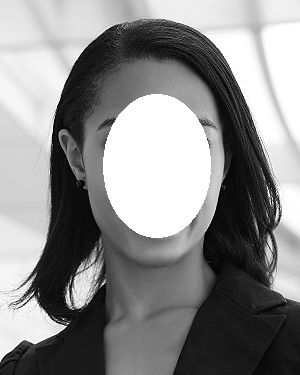
\includegraphics[width=1in,height=1.25in,clip,keepaspectratio]{a1.png}}]{First A. Author} (Fellow, IEEE) and all authors may include 
biographies. Biographies are
often not included in conference-related papers.
This author is an IEEE Fellow. The first paragraph
may contain a place and/or date of birth (list
place, then date). Next, the author’s educational
background is listed. The degrees should be listed
with type of degree in what field, which institution,
city, state, and country, and year the degree was
earned. The author’s major field of study should
be lower-cased.

The second paragraph uses the pronoun of the person (he or she) and
not the author’s last name. It lists military and work experience, including
summer and fellowship jobs. Job titles are capitalized. The current job must
have a location; previous positions may be listed without one. Information
concerning previous publications may be included. Try not to list more than
three books or published articles. The format for listing publishers of a book
within the biography is: title of book (publisher name, year) similar to a
reference. Current and previous research interests end the paragraph.

The third paragraph begins with the author’s title and last name (e.g.,
Dr. Smith, Prof. Jones, Mr. Kajor, Ms. Hunter). List any memberships in
professional societies other than the IEEE. Finally, list any awards and work
for IEEE committees and publications. If a photograph is provided, it should
be of good quality, and professional-looking.
\end{IEEEbiography}

\begin{IEEEbiographynophoto}{Second B. Author,} photograph and biography not available at the
time of publication.
\end{IEEEbiographynophoto}

\begin{IEEEbiographynophoto}{Third C. Author Jr.} (Member, IEEE), photograph and biography not available at the
time of publication.
\end{IEEEbiographynophoto}

\end{document}
